\subsection{Recordings}
\label{sec:recordings}

\textit{Recording site}: To gain information about the habitats of different species of weakly electric fish, we did field recordings in in a tropical grassland plain in the Rio Canocamoa, which is located in the LLanos of the Orinoco basin in the Reserva el Caduceo, San Martín, Departement del Meta in Colombia (fig.~\ref{fig:map}). This area is composed of branched networks of smaller streams and larger rivers.
The measured habitats were chosen dependent on their individual characteristics to gain as much habitat diversity as possible. Thus the habitats varied in water depth, water flow and structure of the ground and the shoreline. During the recording period in early October, right after the rain season, the average water temperature was 25.6 \rpm \ang{1.02}C. The average water conductivity was 9.78 \rpm 4.48 $\frac{\mu S}{cm}$.

\begin{figure}[H]
    \centering
    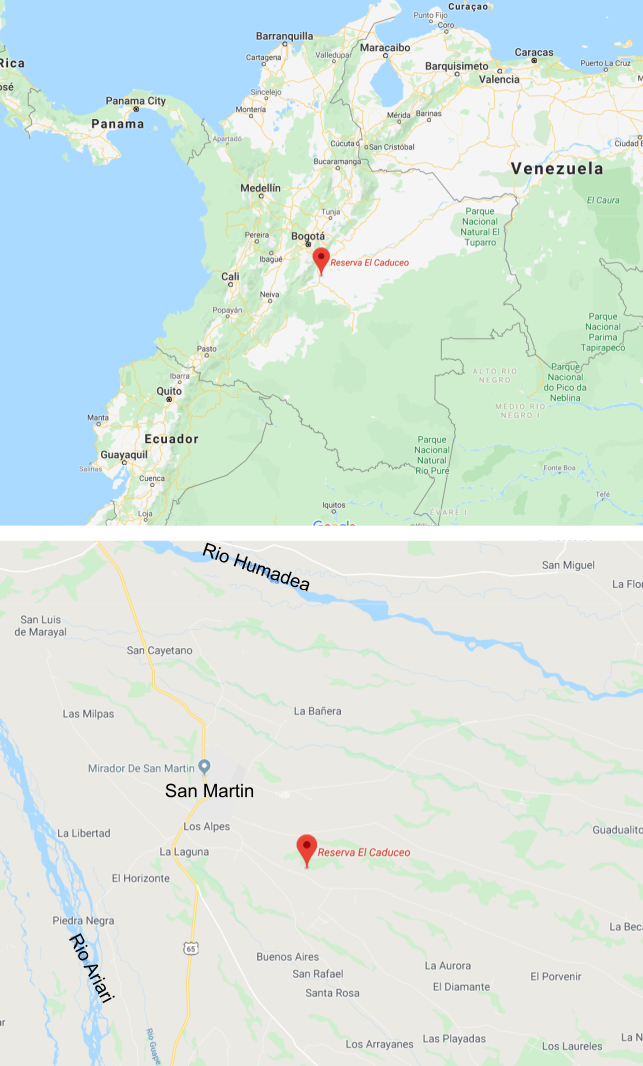
\includegraphics[width=0.58\textwidth]{pictures/Methods/map.png}
    \caption{\textbf{Location Reserva el Caduceo, Colombia.} \textbf{Top:} Location of the Reserva el Caduceo (red) within Colombia. \textbf{Bottom:} Location of the reservation within the Orinoco basin. \url{(https://goo.gl/maps/J3h9ntWjrADx44Sx6, 29.01.2020)}}
    \label{fig:map}
\end{figure}{}

\textit{Recording procedure}: In order to record the electric fields of the fish, self-made fishfinder were used. These consisted of a PVC-rod with an lead electrode on the top and a reference electrode on the bottom (fig.~\ref{fig:fishfinder}). The recorded signal was amplified with an audio amplifier of the brand RadioShack, and recorded via a MP3 player (Trancend’s MP330).
In case of many fish all-around the habitat, the recordings were made systematically, every 1-2 m (fig.~\ref{fig:habitats}~BE). Regular distances were chosen to avoid resampling of individual fish and to cover larger areas. Also, the fishfinder was positioned close to one fish within these recording areas. In case of only a few fish within the habitat, the recordings were made at the positions of each fish (fig.~\ref{fig:habitats}~ACD). Each individual recording within a habitat refers to a micro-habitat. For each measurement’s position the micro-habitat’s characteristics, such as the presence or absence of sand, mud, plants, roots and stones, were documented. The stones were further characterised as stacked or not stacked. Furthermore the water depth and the water flow (Advanced Stream Flowmeter by GEOPACKS) was measured. These characteristics were noted for micro-habitats in which fish were found, as well es for for areas without any detectable fish.
Over all, within 13 different habitats, 19 micro-habitats without detectable weakly electric fish and 139 different micro-habitats with weakly electric fish were found, characterised and recorded.

\begin{figure}[H]
    \centering
    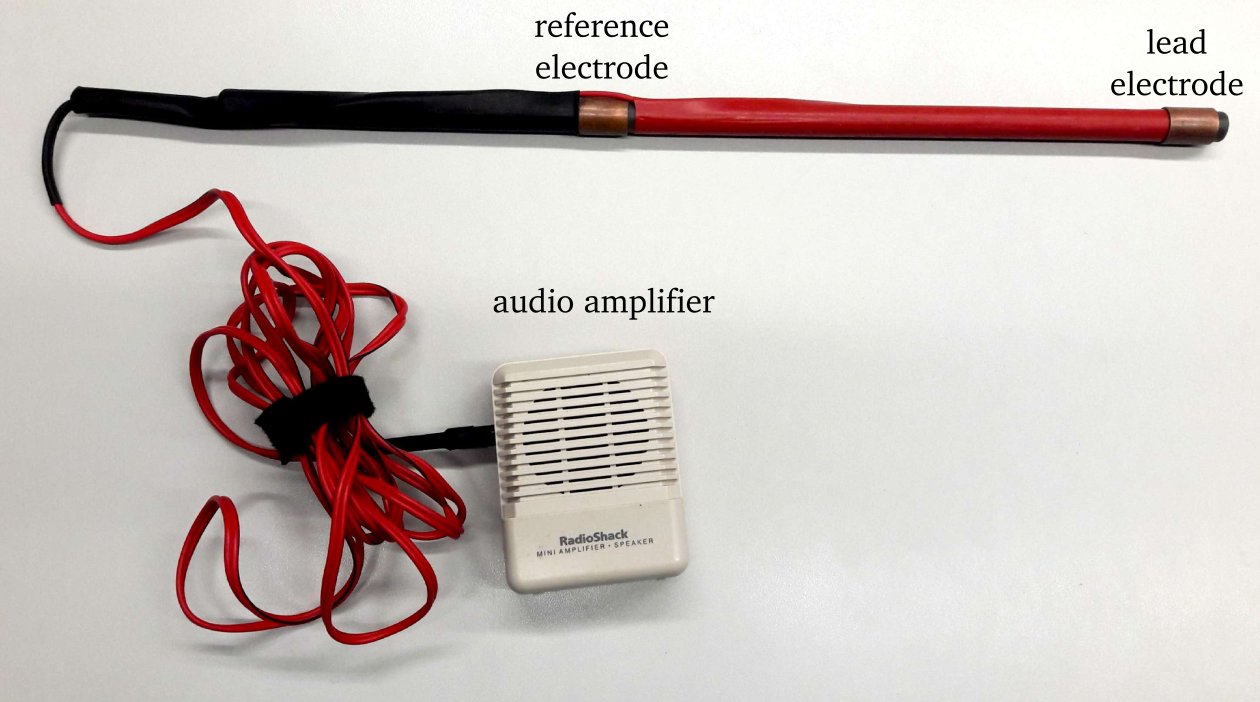
\includegraphics[width=\textwidth]{pictures/Methods/fishfinder.png}
    \caption{\textbf{Self-made fishfinder and audio amplifier of the brand RadioShack}}
    \label{fig:fishfinder}
\end{figure}{}

\begin{figure}[H]
    \centering
    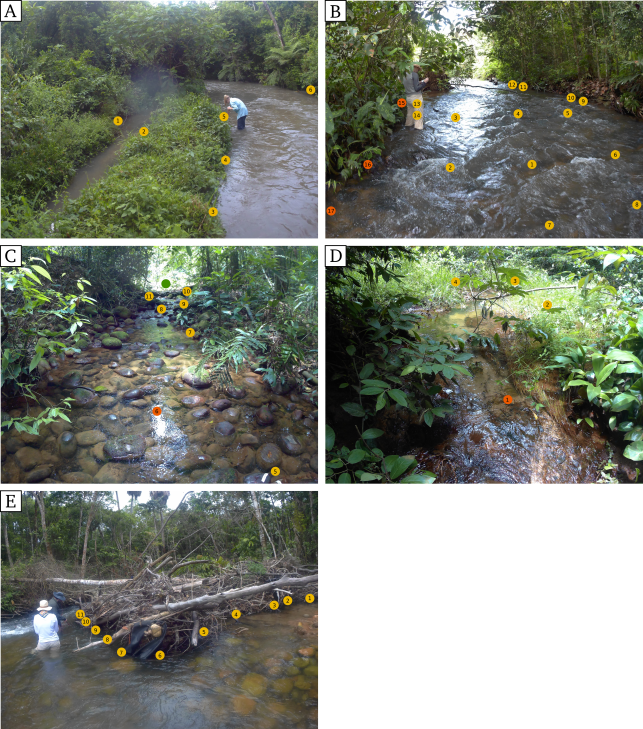
\includegraphics[width = 0.9\textwidth]{pictures/Methods/all_habitats.png}
    \caption{\textbf{Five example recording habitats in the reservoir El Caduceo, with each recording site (micro-habitat). A:} On the left: small muddy side stream with two micro-habitats (yellow dots: 1 \& 2), on the right: large fast river with four recording sides (3~-~6). \textbf{B:} The same river as in A further downstream, with fourteen micro-habitats with fish (yellow) and three micro-habitats without fish (orange, 15~-~17). \textbf{C:} A clear, stony side stream with six micro-habitats with fish (yellow) and one 'no fish area' (orange, 6). The adjacent habitat D is marked with a green dot. \textbf{D:} Further up in the side stream of habitat C, this habitat is composed of a muddy underground with many plants. In hree of the micro-habitats fish were found (yellow, 2~–~4), in one micro-habitat no fish were found (orange, 1). \textbf{E:} Eleven recording sites systematically along a wooden dam in a large river.}
    \label{fig:habitats}
\end{figure}

\subsection{Sorting Species}
In order to analyse the (micro-)habitat preference of different species of weakly electric fish, the first task was to determine how many fish were actually in each of  the recordings. Therefore, with the program thunderfish ($\copyright$ Benda-Lab) each recording was analysed and based on the power spectrum, the EOD and waveform for each individual fish was calculated.
Dependent on the EOD waveform the fish were categorised into wave- and pulse-type fish. Pulse-type fish weren't further separated into different species. To further separate the wave-type fish into different species, different EOD parameters were extracted with the program collectfish ($\copyright$ Benda-Lab). On the basis of the EOD frequency and the relative peak amplitude (RPA), the fish's EOD were separated into three clusters, each corresponding to one endemic species: \textit{Apteronotus macrostomus} \citep{Santana2013}, \textit{Sternopygus macrurus} \citep{Keller1991} and \textit{Eigenmannia virescens}~\citep{silva2009cytogenetic}. According to the literature the EODf of Sternopygus ranges from 50~-~200~Hz \citep{Keller1991}, the EODf of \textit{Eigenmannia} from 250~-~600~Hz \citep{Hopkins_74}, while the EODf of adult Apteronoti ranges from 600~-~1000~Hz. The EODf of juvenile Apteronoti ranges from 400 to 600~Hz \citep{Meyer1987}.
Within the critical EODf window of 250~-~577~Hz, where the EOD frequencies of \textit{Apteronotus} and \textit{Eigenmannia} overlap, the fish species couldn't be determined easily. Since both species differ in their EOD waveform, waveform characteristics were used to discriminate between these two species within the critical range: The waveform of \textit{Eigenmannia} and \textit{Apteronotus} differ in the aspect of the relative peak amplitude (RPA). The RPA of \textit{Apteronotus} is more or less 1, since the EOD is a biphasic signal \citep{Zupanc_Bullock_2005} (fig.~\ref{fig:EOD_waveforms}). The waveform of \textit{Eigenmannia}, however, is monophasic \citep{Zupanc_Bullock_2005} with a slightly shifted zero line towards the negative. Therefor, the amplitude of the minimum is about the half of the amplitude of the maximum. Consequently, the RPA of \textit{Eigenmannia} is 0.5 (fig.~\ref{fig:EOD_waveforms}). Based on the distribution of the clusters and the waveform characteristics, the boundary was placed at a relative peak amplitude of 0.72 (fig.~\ref{fig:cluster}). However, regarding the waveforms of the individual Apteronoti with EOD frequencies below 500~Hz, the waveforms did not show the typal characteristics. Accordingly, these individuals were excluded from further analysis. Since only two individuals of the genus Sternopygus were recorded, these individuals were also excluded from the analysis.

%%\item  \textcolor{gray}{how many fish of a given species were present in each of the \textcolor{red}{???} recordings. Therefor, for each individual fish of each recording the EOD characteristics were analyzed with/by the program thunderfish ($\copyright$ Benda-Lab).   Within an analyzing window of 8s this program calculates the average EOD waveform (n=1000) and its power spectrum for each individual fish. Individuals with a power less then -60 dB were not analyzed.   Waveforms of fish, that were orientated tail first to the recording electrodes, were flipped in amplitude. For the pulse-fish only the EOD frequency (EODf) was analyzed.  For the wave-fish EOD parameters, such as fundamental or EOD frequency, frequency of the harmonics and their amplitudes and phases, were calculated. Other EOD characteristics, i.e. peak to peak amplitude, relative peak amplitudes and peak to peak distance  then: plot this characteristics against each other to search for clusters to determine species habitat characteristica + species for each individual fish in the recordings wave-type fish  Apteronotus leptorhynchus EODf: 600-1100 Hz (Meyer, 1973 and \cite{Hopkins_74}) ! juveniles lower in EODf: can be down to 400-500 Hz (Meyer, 1973) Eigenmannia EODf: 240-600 Hz (Meyer, 1973 and \cite{Hopkins_74}) Sternopygus EODf: 50-150 Hz (Meyer, 1973 and \cite{Hopkins_74}) Critical Freqency = 400 – 600 Hz (Eigenmannia vs. Apteronotus) to determine which waveform belongs to which species, different waveform characteristics were plotted against each other  Parameter 1 (EODf): Sterno < 250 Hz < Eigenmannia < 577 Hz < Apteronotus Parameter 2 (relative peak amplitude): amplitude of minimum relative to amplitude of maximum 72 \% Within the critical EODf window of 250~-~577~Hz the fish species couldn't be determined easily. The waveform of Eigenmannia and Apteronotus differ in the aspect of the relative peak amplitude, regarding that the relative peak amplitude of Apteronotus is more or less 1 since it is a biphasic (\textcolor{red}{Quelle}) signal around 0 (\textcolor{red}{Quelle}). The waveform of Eigenmannia however, is monophasic (\textcolor{red}{Quelle}) with a slightly shifted zero line towards the negativ (\textcolor{red}{Quelle}). Therefore the amplitude of the minima is about the half of the amplitude of the maxima.}

\begin{figure}[H]
    \centering
    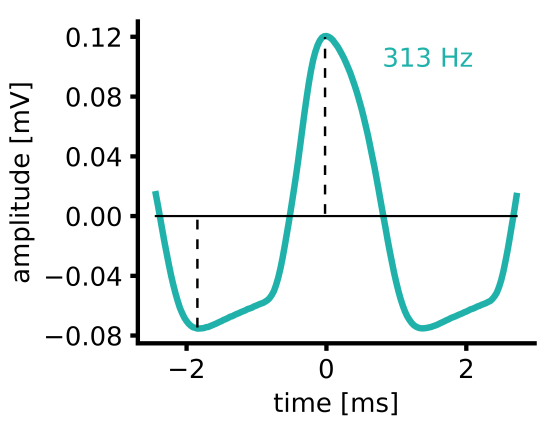
\includegraphics[width=0.496\textwidth]{pictures/Methods/waveform_eig.png}
    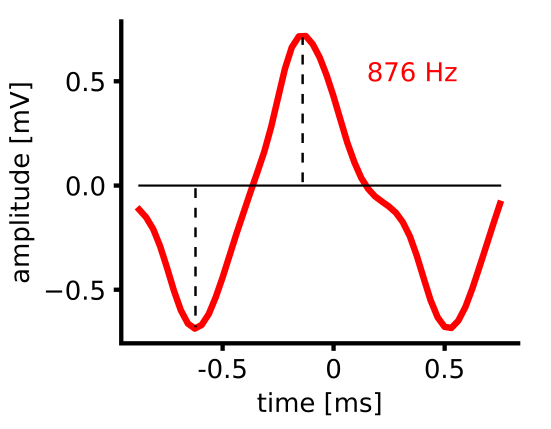
\includegraphics[width=0.496\textwidth]{pictures/Methods/waveform_apt.png}
    \caption{\textbf{EOD waveform of \textit{Apteronotus} and \textit{Eigenmannia}.} Shown are exemplary EOD waveforms of individuals of the species \textit{Eigenmannia} (cyan), with an EOD frequency of 313~Hz, and \textit{Apteronotus} (red), with an EODf of 876~Hz. The amplitudes of the positive and negative peaks are marked with dashed lines.}
    \label{fig:EOD_waveforms}
\end{figure}{}

\begin{figure}[H]
    \centering
    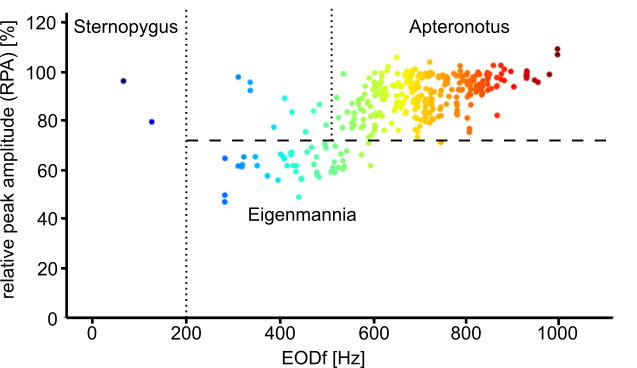
\includegraphics[width=0.9\textwidth]{pictures/Methods/cluster.png}
    \caption{\textbf{Determination of wave-type species dependent on RPA and EODf.} Shown is the relative peak amplitude (RPA) and the EOD frequency of each recorded animal. The color corresponds to the EODf. Fish with a EODf lower than 200~Hz were identified as Sternopygus. The differentiation between \textit{Apteronotus} and \textit{Eigenmannia} was based on the RPA. Animals with a RPA lower than 0.72 were classified as \textit{Eigenmannia}. Animals with a RPA greater than 0.72 as \textit{Apteronotus}. Since, the waveform of the Apteronoti with an EODf lower than 500~Hz was typal, these individuals were excluded from further analysis.}
    \label{fig:cluster}
\end{figure}{}